\section{Date: 2026-08-28}
\noindent \textbf{Series ID: WPU39} 

\noindent This series is titled Producer Price Index by Commodity: Credit Intermediation Services (Partial) and has a frequency of Monthly. The units are Index Jun 2009=100 and the seasonal adjustment is Not Seasonally Adjusted.The observation start date is 2009-06-01 and the observation end date is 2026-07-01.The popularity of this series is 2. \\ 

\noindent \textbf{Series ID: 4522MPCSMN} 

\noindent This series is titled Advance Retail Sales: Department Stores and has a frequency of Monthly. The units are Percent Change from Preceding Period and the seasonal adjustment is Not Seasonally Adjusted.The observation start date is 1992-02-01 and the observation end date is 2026-07-01.The popularity of this series is 1. \\ 

\subsection{Raw Regression}
\noindent Regresses the two series against each other directly. A significant result here can come just as easily from both series sharing a long-run trend as from any real relationship.

\begin{center}
\begin{tabular}{lclc}
\toprule
\textbf{Dep. Variable:}     & value\_fred\_4522MPCSMN & \textbf{  R-squared:         } &     0.007   \\
\textbf{Model:}             &           OLS           & \textbf{  Adj. R-squared:    } &     0.002   \\
\textbf{Method:}            &      Least Squares      & \textbf{  F-statistic:       } &     1.349   \\
\textbf{Date:}              &     Fri, 28 Aug 2026    & \textbf{  Prob (F-statistic):} &    0.247    \\
\textbf{Time:}              &         21:35:13        & \textbf{  Log-Likelihood:    } &   -1090.0   \\
\textbf{No. Observations:}  &             206         & \textbf{  AIC:               } &     2184.   \\
\textbf{Df Residuals:}      &             204         & \textbf{  BIC:               } &     2191.   \\
\textbf{Df Model:}          &               1         & \textbf{                     } &             \\
\textbf{Covariance Type:}   &        nonrobust        & \textbf{                     } &             \\
\bottomrule
\end{tabular}
\begin{tabular}{lcccccc}
                            & \textbf{coef} & \textbf{std err} & \textbf{t} & \textbf{P$> |$t$|$} & \textbf{[0.025} & \textbf{0.975]}  \\
\midrule
\textbf{const}              &      38.6856  &       28.473     &     1.359  &         0.176        &      -17.453    &       94.824     \\
\textbf{value\_fred\_WPU39} &      -0.3398  &        0.293     &    -1.161  &         0.247        &       -0.917    &        0.237     \\
\bottomrule
\end{tabular}
\begin{tabular}{lclc}
\textbf{Omnibus:}       & 347.731 & \textbf{  Durbin-Watson:     } &     2.210  \\
\textbf{Prob(Omnibus):} &   0.000 & \textbf{  Jarque-Bera (JB):  } & 86896.432  \\
\textbf{Skew:}          &   8.253 & \textbf{  Prob(JB):          } &      0.00  \\
\textbf{Kurtosis:}      & 102.254 & \textbf{  Cond. No.          } &      824.  \\
\bottomrule
\end{tabular}
%\caption{OLS Regression Results}
\end{center}

Notes: \newline
 [1] Standard Errors assume that the covariance matrix of the errors is correctly specified.

\begin{figure}
\centering
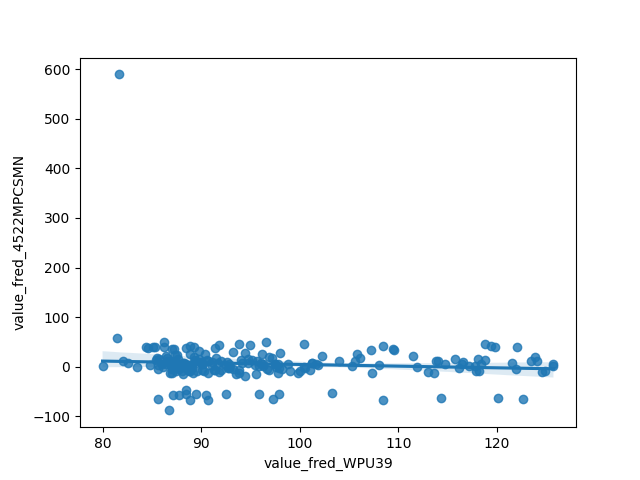
\includegraphics[scale = 0.9]{plots/plot_2026-08-28.png}
\caption{Raw Regression Plot for 2026-08-28}
\end{figure}
\newpage
\subsection{Detrended Regression}
\noindent Regresses the residuals of each series after removing its own linear time trend, so a shared trend can no longer drive the result on its own. A relationship that stays significant here is better evidence of a genuine link between the two series.

\begin{center}
\begin{tabular}{lclc}
\toprule
\textbf{Dep. Variable:}                & value\_fred\_4522MPCSMN\_detrended & \textbf{  R-squared:         } &     0.014   \\
\textbf{Model:}                        &                OLS                 & \textbf{  Adj. R-squared:    } &     0.009   \\
\textbf{Method:}                       &           Least Squares            & \textbf{  F-statistic:       } &     2.884   \\
\textbf{Date:}                         &          Fri, 28 Aug 2026          & \textbf{  Prob (F-statistic):} &   0.0910    \\
\textbf{Time:}                         &              21:35:14              & \textbf{  Log-Likelihood:    } &   -1089.1   \\
\textbf{No. Observations:}             &                  206               & \textbf{  AIC:               } &     2182.   \\
\textbf{Df Residuals:}                 &                  204               & \textbf{  BIC:               } &     2189.   \\
\textbf{Df Model:}                     &                    1               & \textbf{                     } &             \\
\textbf{Covariance Type:}              &             nonrobust              & \textbf{                     } &             \\
\bottomrule
\end{tabular}
\begin{tabular}{lcccccc}
                                       & \textbf{coef} & \textbf{std err} & \textbf{t} & \textbf{P$> |$t$|$} & \textbf{[0.025} & \textbf{0.975]}  \\
\midrule
\textbf{const}                         &   -4.971e-12  &        3.349     & -1.48e-12  &         1.000        &       -6.603    &        6.603     \\
\textbf{value\_fred\_WPU39\_detrended} &      -0.5656  &        0.333     &    -1.698  &         0.091        &       -1.222    &        0.091     \\
\bottomrule
\end{tabular}
\begin{tabular}{lclc}
\textbf{Omnibus:}       & 344.090 & \textbf{  Durbin-Watson:     } &     2.224  \\
\textbf{Prob(Omnibus):} &   0.000 & \textbf{  Jarque-Bera (JB):  } & 83116.692  \\
\textbf{Skew:}          &   8.093 & \textbf{  Prob(JB):          } &      0.00  \\
\textbf{Kurtosis:}      & 100.065 & \textbf{  Cond. No.          } &      10.1  \\
\bottomrule
\end{tabular}
%\caption{OLS Regression Results}
\end{center}

Notes: \newline
 [1] Standard Errors assume that the covariance matrix of the errors is correctly specified.

\begin{figure}
\centering
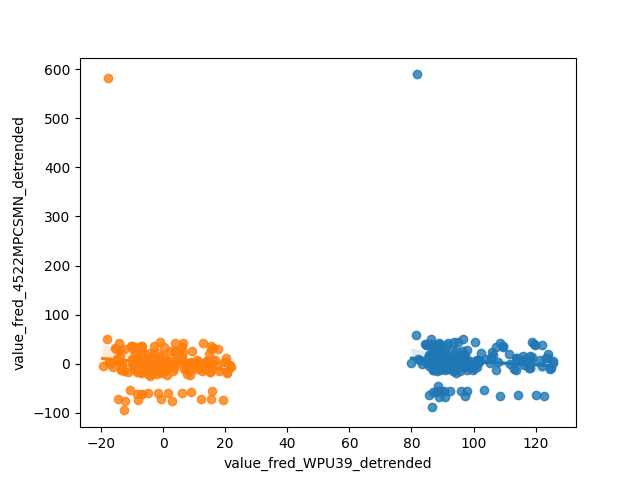
\includegraphics[scale = 0.9]{plots/plot_2026-08-28_detrended.png}
\caption{Detrended Regression Plot for 2026-08-28}
\end{figure}
\newpage
